\chapter{Introduction}

\epigraph{Me caí, me paré, caminé, me subí \\ me fui contra la corriente \\ y también me perdí}{Soy Yo \\ Bomba Estéreo, 2015}

\section{Context}

This thesis is the capstone project of my master's program, between the academic years 2019-2021 at MIT Media Lab, where I am a Research Assistant at the groups Opera of the Future and Future Sketches. The work presented here has been developed mostly while working remotely from my room in Boston MA during the COVID19 pandemic.

This thesis is a collection of media arts instruments made with microcontrollers and \acrfull{ML}, with a strong emphasis on \acrfull{AI} ethics and \acrfull{DIY} methods. Its main audience is beginners and artists, and it is my hope that this work can inspire a new generation of instrument makers, artists, designers, educators, programmers, policy makers, activists, and enthusiasts.

\begin{figure}[ht]
  \centering
  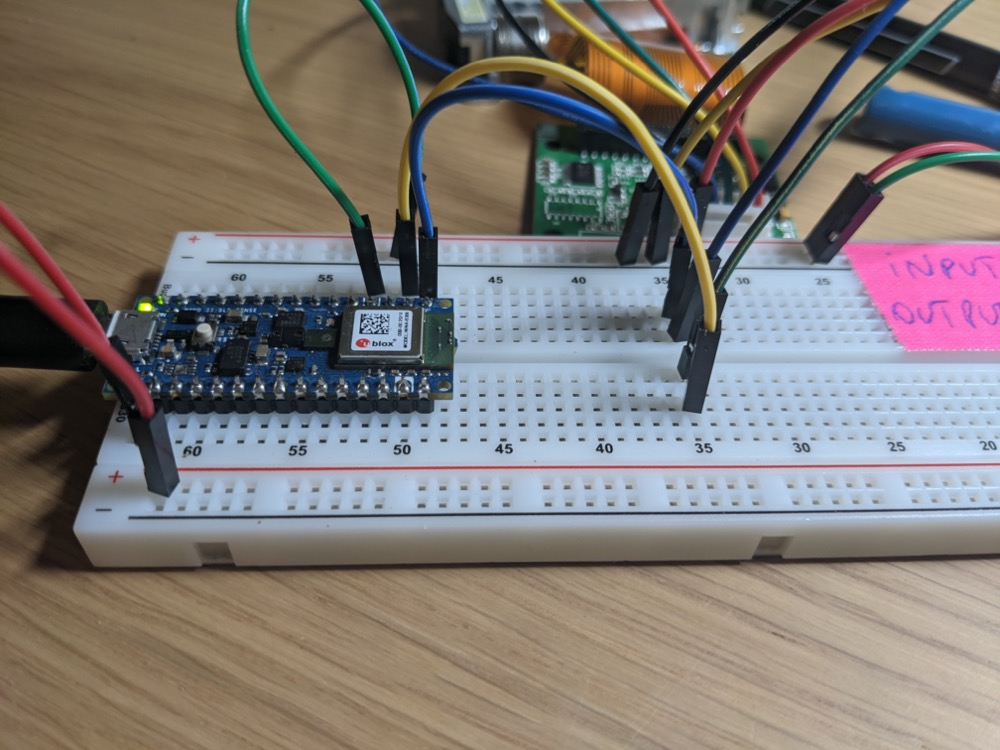
\includegraphics[width=0.75\linewidth,height=0.25\textheight,keepaspectratio]{images/tiny-trainable-instruments-early-protoype.jpg}
  \caption{Early prototype of Tiny trainable instruments}
  \caption*{Picture taken by myself}
  \label{fig:tiny-trainable-instruments-early-protoype}
\end{figure}

\acrshort{ML} has several barriers of entry, including cost, complexity, and difficulty. Since my practice is based on sharing and working on the open with different communities, I am not a fan of the current state of industrial \acrshort{ML} that relies on proprietary software and hardware. This tends to happen because their ML models are aiming for high precision, and need to be trained for long periods of time, using expensive non open computational resources, with huge datasets that often are scraped from the internet without the explicit consent of the people, and a byproduct of surveillance capitalism.

TODO: insert picture of surveillance camera near my home, in the middle of nature.

The release of the library Arduino TensorFlow Lite in late 2019 made me aware of the tiny \acrshort{ML} field, a subset of \acrshort{ML} that focuses on hardware and software that are able to run calculations both on-device and with low power, a stark contrast to many industrial \acrshort{ML} applications. The tutorials published by Arduino showed how to build your own database to detect colors and gestures, and I decided that this thesis project would be an exploration of the artistic applications of these emerging techniques.

One aspect that deeply resonated with me was \textbf{data agency}, the ability to capture my own data, and use it for my own purposes, in the microcontroller, without having to rely on databases, and bypassing any corporate or government surveillance. Since during this thesis work and pandemic lockdown context, I have found myself several times during the year working in my room on my own, capturing data of myself, and then building databases for other people to use, in a way that reminds of one of my favorite artists and activists, Ai Weiwei, who in 2012 while facing government surveillance, decided to livestream all his activites from his house, which I think it's a way of reclaiming agency about your data. 

\begin{figure}[ht]
  \centering
  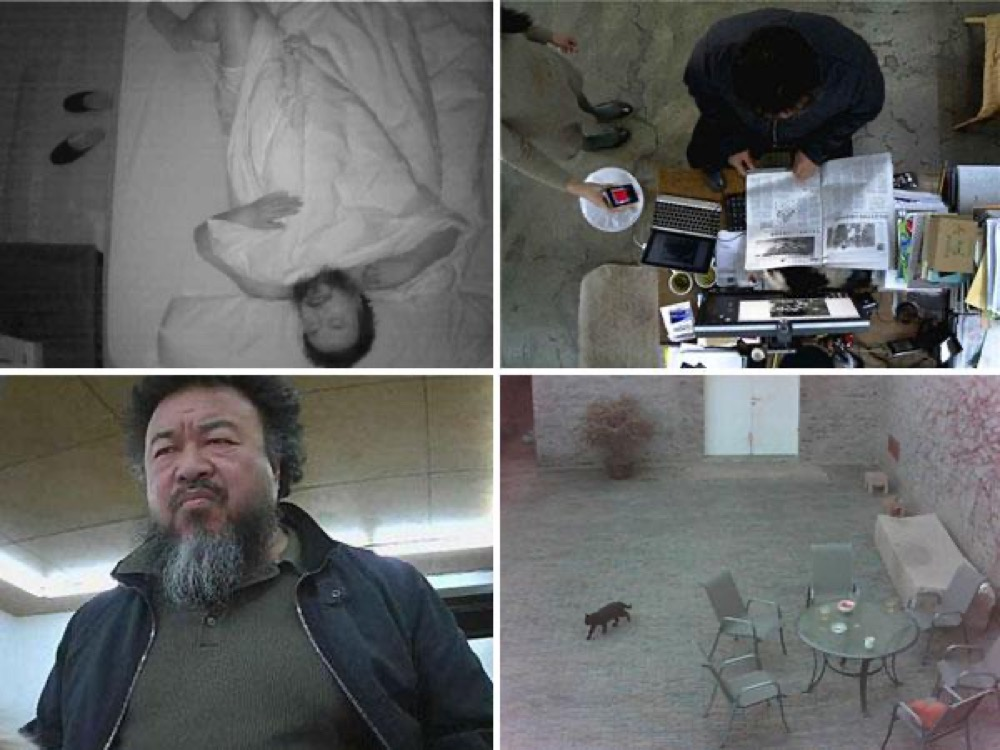
\includegraphics[width=0.75\linewidth,height=0.25\textheight,keepaspectratio]{images/weiweicam.jpg}
  \caption{Weiweicam, by Ai Weiwei, 2012}
  \caption*{Retrieved from \cite{website-forbes-ai-weiwei-cam}}
  \label{fig:weiweicam}
\end{figure}

I am an underrepresented minority, and often it happens to me that supposedly automatic neutral technologies don't understand me. Here is an example of the popular software Zoom, where I spoke out loud "This is a test to show that Zoom speech to text transcription does not work with my voice because of my accent", but the words Zoom and voice were transcribed as soon and boys, respectively.

\begin{figure}[ht]
  \centering
  
\includegraphics[width=0.75\linewidth,height=0.25\textheight,keepaspectratio]{images/zoom-introduction.jpg}
  \caption{Screen capture of speech to text on Zoom, introduction}
  \caption*{Screen capture by myself}
  \label{fig:zoom-voice}
\end{figure}

Here is also a further experiment of pronunciation with less common words, the names of the members of my thesis commitee: Tod Machover, Mitchel Resnick, Zach Lieberman, where the result had even more errors.

\begin{figure}[ht]
  \centering
  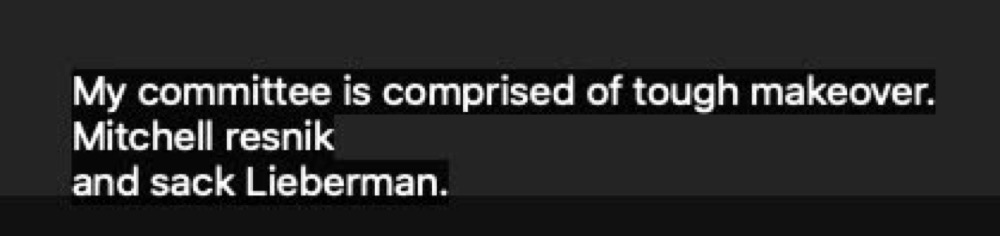
\includegraphics[width=0.75\linewidth,height=0.25\textheight,keepaspectratio]{images/zoom-commitee.jpg}
  \caption{Screen capture of speech to text on Zoom, committee}
  \caption*{Screen capture by myself}
  \label{fig:zoom-committee}
\end{figure}

These examples are not affecting me negatively, but these algorithmic decisions can have devastating effects in equity and discrimination.  Despite \acrshort{ML} algorithms being promoted by corporations and governments as unbiased, most probably these algorithms have never been exposed to Chilean people with my accent.

\begin{figure}[ht]
  \centering
  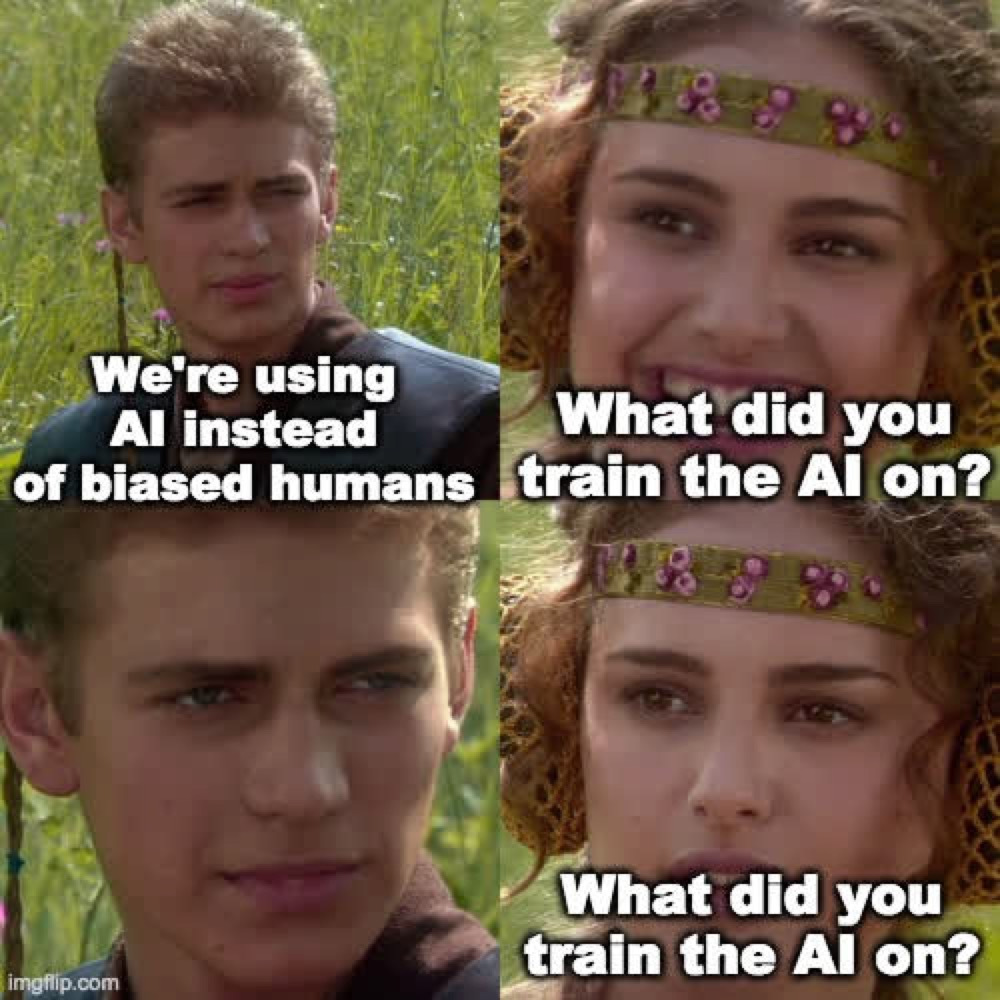
\includegraphics[width=0.75\linewidth,height=0.25\textheight,keepaspectratio]{images/meme-star-wars.jpg}
  \caption{Meme about biased data}
  \caption*{Retrieved from \cite{website-twitter-janellecshane-meme}}
  \label{fig:meme-star-wars}
\end{figure}

Because of these errors, but more importantly, because of me renouncing to my privacy I routinously turn off voice assistants and text completion in my devices (if you have ever interacted with me over text, I typed every single character :)), and tape the camera of my computer.

Not always we can just turn off or opt out of these computational or \acrshort{AI} systems, but we should be able to, because there is even more at stake than losing our privacy! We could be subjected to the harmful \textbf{algorithmic bias}. As the Algorithmic Justice League explains on their website:

\begin{displayquote}
In today’s world, AI systems are used to decide who gets hired, the quality of medical treatment we receive, and whether we become a suspect in a police investigation. While these tools show great promise, they can also harm vulnerable and marginalized people, and threaten civil rights. Unchecked, unregulated and, at times, unwanted, AI systems can amplify racism, sexism, ableism, and other forms of discrimination.\cite{website-algorithmic-justice-league}
\end{displayquote}

I highly recommend everyone to watch the Coded Bias documentary on Netflix, and inform themselves about the important and necessary digital advocacy of the Algorithmic Justice League, who have helped me learn the language to navigate these important topics of civil rights.

The final catalyst that led me to this thesis happened a year ago, when I watched a video \cite{website-talk-technology-and-public-art-rafael-lozano-hemmer} of a conversation between artists Rafael Lozano-Hemmer and Dorothy Santos, and on 36m28s Rafael said " Face recognition needs to be banned in all applications except art."

This was the perfect spark for starting to work on this project, and make more accesible these computational techniques to beginners, enthusiasts, and educators. Despite the creative anda artistic applications that I will show during this thesis, let's keep in mind that as \acrshort{ML} becomes cheaper and more pervasive, it is not the solution to all problems, or even needed in many scenarios.

\begin{figure}[ht]
  \centering
  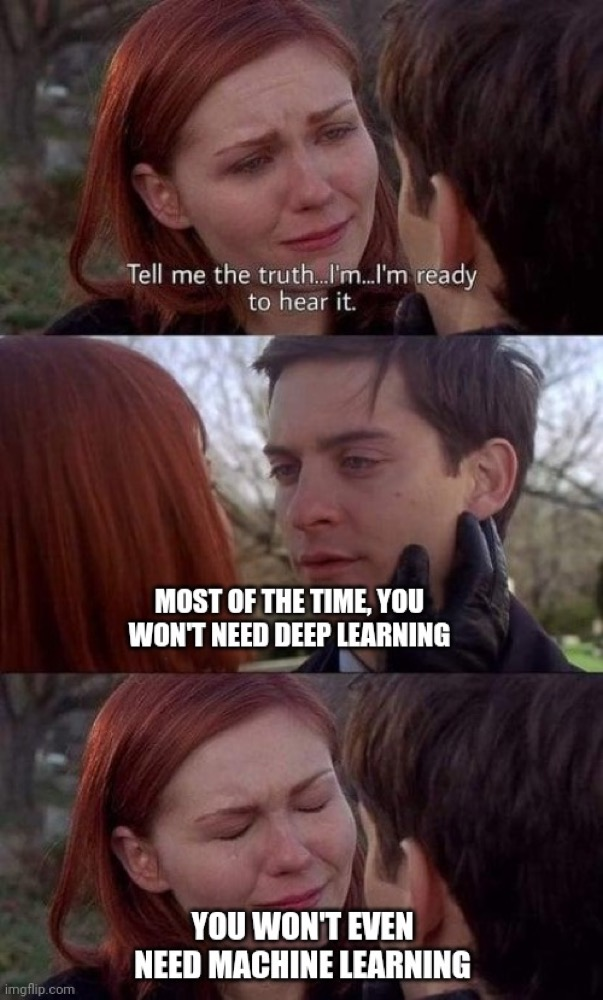
\includegraphics[width=0.75\linewidth,height=0.40\textheight,keepaspectratio]{images/meme-spider-man.jpg}
  \caption{Meme about need of machine learning}
  \caption*{Retrieved from \cite{website-twitter-dynamicwebpaige-meme}}
  \label{fig:meme-spider-man}
\end{figure}

In this XXIth century artists have an unprecedented access to tools for making new tools and instruments, and I intend this thesis to be a foundation for a new generation of instrument makers for manipulating audiovisual material, using \acrshort{ML}. This approach is really exciting because it allows beginners and artists to train their instruments instead of programming them, by inputting data for tuning, instead of having to write lines of code and fixed thresholds for changing their behavior.

\section{Objectives and dreams}

Infrastructure and cooperation are key to society, I love how I can bike on roads and hike on paths that were built as shared resources for the benefit of everyone, and I hope this work can be adopted by fellow artists and educators to create new instruments for arts, and to inspire critical and ethical thinking about \acrshort{AI}

I am convinced there is a huge educational value in creating your own databases, and in this thesis I propose techniques and software so that people can build their own databases, in order to train models that are tailored to each person's voice or environment, instead of using widespread databases and their inherent biases. Also I hope this work will help appreciate the craft of making databases, or even the exploitation and problematic lack of consent behind them.

Finally, as a non USA citizen subjected to all sorts of regulations during my studies here, and as a programmer working with software with various licenses, and as musician repurposing other's people's work via sampling, I know first hand that navigating legal documents is very hard. As an anecdote, in 2010, GameStation added a soul clause to their terms of conditions as an April Fool's prank, making them legal owners of thousands of customers' souls \cite{website-huffpost-gamestation-soul-clause}. And back in 2007, it was estimated that people would need around 250 hours every year to actually read the privacy policies shown to them \cite{article-cost-of-reading-privacy-policies}. That is why in this thesis I tried my best to cite every work that I am both using as a building block, or served as a direct or indirect inspiration.

I hope this work can be taken to the next step, by building a new generation of private and smart devices, like one of my first dreams, a drum machine I can talk to, and ask for different rhythms mid performance, or using my body gestures to write poems.

\section{Thesis outline}

This thesis has cover the following chapters:

\begin{enumerate}
  \item Chapter 1, Introduction: the context and summary of this thesis.
  \item Chapter 2, Tiny trainable instruments: description of the design strategies for the software and hardware, description of the support team working on this thesis.
  \item Chapter 3, Early experiments: my earlier work that led to this thesis, in the topics of media arts education, microcontrollers, and \acrshort{ML}, among others.
  \item Chapter 4, Background and inspiration: work by other people which has informed my work.
  \item Chapter 5, Project evaluation: user feedback, field notes.
  \item Chapter 6, Conclusions and future work: next iterations of the instruments, and their proposed use for educators and artists.
  \end{enumerate}
